\newpage
\pagestyle{fancy}
\lhead{\textsc{Chapitre 4. Application décisionnelle et intégration des modèles prédictifs}}
\renewcommand{\headrulewidth}{0.5pt}
\renewcommand{\footrulewidth}{0.5pt}
 
\chapter{Application décisionnelle et intégration des modèles prédictifs}\setlength{\headheight}{28pt}
\label{ch4}
\minitoc
\newpage
 
\section{Introduction}
 
Au cours du chapitre précédent, nous avons mis en place une infrastructure décisionnelle complète permettant d'explorer, d'analyser et de visualiser les données de BIOSPHERE à travers des tableaux de bord interactifs développés avec Power BI. Cette couche de Business Intelligence constitue une avancée importante pour l'entreprise, puisqu'elle transforme les données opérationnelles en indicateurs structurés facilitant le pilotage des ventes, des achats et du stock.
 
Cependant, malgré l'intérêt de cette approche descriptive, les dashboards présentent une limite majeure : ils permettent d'observer les phénomènes critiques une fois qu'ils se sont produits, sans offrir de capacité d'anticipation. À titre d'exemple, les tableaux de bord de suivi du stock mettent en évidence un nombre élevé d'articles en rupture, estimé à 3~994 produits au 30 juillet 2025. 
 
De plus, la gestion des niveaux de stock repose encore principalement sur des règles manuelles et l'expérience métier. En l'absence de mécanismes prédictifs, il devient difficile d'identifier les produits à risque, d'anticiper les besoins de réapprovisionnement ou de détecter les évolutions anormales du comportement du stock.
 
Dans ce contexte, l'intégration d'une approche Data Science devient essentielle afin de faire évoluer le système décisionnel vers une logique proactive et prédictive. L'objectif principal de ce chapitre est donc d'exploiter l'historique des données de stock afin de construire des modèles capables d'anticiper les ruptures futures et d'estimer les niveaux de stock à venir.
 
Pour répondre à cette problématique, deux axes analytiques complémentaires ont été retenus :
 
\begin{itemize}
    \item Un axe de classification visant à prédire le risque de rupture de stock pour chaque produit et chaque période future ;
    \item Un axe de régression visant à estimer quantitativement le niveau futur du stock sur un horizon donné.
\end{itemize}
 
Ces deux approches ne sont pas redondantes mais complémentaires. La classification permet d'identifier l'existence d'un risque, tandis que la régression en mesure l'ampleur potentielle. Ensemble, elles constituent un système d'aide à la décision permettant une gestion plus intelligente, proactive et optimisée des stocks.
 
Ce chapitre présente ainsi l'ensemble du pipeline de Data Science mis en œuvre, depuis la préparation des données et la construction des variables jusqu'à l'entraînement, la validation et l'analyse critique des modèles prédictifs développés.
 
\section{Section 1 : Cadre méthodologique du Sprint 4}
 
\subsection{Positionnement du Sprint dans la méthodologie SCRUM}
 
Le développement du projet BIOSPHERE a été structuré selon une approche agile basée sur la méthodologie SCRUM. Cette organisation a permis de découper le projet en plusieurs sprints successifs, chacun correspondant à un ensemble cohérent d'objectifs fonctionnels et techniques.
 
Les premiers sprints ont principalement porté sur la mise en place de l'infrastructure décisionnelle de l'entreprise. Ces travaux ont principalement concerné la collecte des données depuis l'ERP, la conception du Data Warehouse, le développement des processus ETL ainsi que la création des tableaux de bord analytiques avec Power BI. L'ensemble de ces étapes a permis de construire une architecture décisionnelle centralisée destinée à l'analyse descriptive des données métier.
 
Dans cette continuité, le Sprint 4 a été consacré à l'intégration de la dimension prédictive et intelligente du système décisionnel. 
 
Ce sprint constitue ainsi une étape stratégique du projet puisqu'il introduit les techniques de Data Science et de Machine Learning afin de répondre à deux problématiques métier majeures :
 
\begin{itemize}
    \item La prédiction des risques de rupture de stock.
    \item L'estimation des niveaux futurs du stock.
\end{itemize}
 
Contrairement aux tableaux de bord descriptifs qui offrent une vision rétrospective de l'activité, les modèles développés dans ce sprint permettent d'orienter la prise de décision vers une logique prédictive et anticipative.
 
\subsubsection{Contexte et évolution vers une approche prédictive}
 
Les trois premiers sprints du projet BIOSPHERE ont permis de mettre en place une infrastructure décisionnelle complète reposant sur un Data Warehouse centralisé et un ensemble de tableaux de bord Power BI destinés au suivi des ventes, des achats et des stocks. Cette plateforme offre aux décideurs une vision consolidée et fiable de l'activité de l'entreprise à travers différents indicateurs de performance.
 
Grâce à cette architecture, les utilisateurs disposent désormais d'un accès structuré aux données et peuvent analyser efficacement les tendances observées ainsi que les performances passées de l'entreprise. Toutefois, cette approche reste principalement descriptive puisqu'elle permet d'expliquer les événements déjà survenus sans fournir d'informations sur les évolutions futures.
 
Dans une logique de maturité analytique, le projet évolue ainsi vers une nouvelle étape consistant à intégrer des capacités prédictives au système décisionnel. L'objectif n'est plus uniquement de comprendre le passé, mais également d'anticiper les comportements futurs afin de soutenir la prise de décision. Cette évolution constitue l'objectif principal du Sprint 4, consacré à l'intégration de techniques de Data Science et de Machine Learning destinées à enrichir la plateforme décisionnelle par une dimension prédictive.
 
\subsubsection{Objectifs du sprint}
 
Face à ces problématiques, le Sprint 4 a été orienté vers le développement d'un pipeline de Data Science capable d'anticiper les comportements futurs du stock à partir des données historiques disponibles.
 
Les principaux objectifs de ce sprint sont les suivants :
 
\begin{itemize}
    \item Développer un modèle de classification permettant de prédire les risques de rupture de stock.
    \item Développer un modèle de régression permettant d'estimer les niveaux futurs du stock.
    \item Construire un pipeline de préparation et de transformation des données adapté aux séries temporelles.
\end{itemize}
 
L'objectif global de ce sprint est ainsi de transformer le système décisionnel existant en une plateforme capable non seulement d'analyser les données passées, mais également d'anticiper les risques futurs afin d'améliorer la gestion opérationnelle du stock.
 
\begin{table}[H]
\centering
\caption{Sprint 4 : Pipeline Data Science : Prévision de stock}
\label{tab:ch4:sprint4}
\resizebox{\textwidth}{!}{
\begin{tabular}{|p{3.5cm}|p{2.5cm}|p{1.5cm}|p{2.5cm}|p{3.5cm}|}
\hline
\multicolumn{1}{|c|}{\textbf{Sprint / Phase}} & 
\multicolumn{1}{c|}{\textbf{User Stories}} & 
\multicolumn{1}{c|}{\textbf{Priorité}} & 
\multicolumn{1}{c|}{\textbf{Durée estimée}} & 
\multicolumn{1}{c|}{\textbf{Livrable attendu}} \\
\hline
Sprint 4 : Pipeline Data Science : Prévision de stock & US02, US03, US05, US08 & Haute & 2 semaines & Modèles prédictifs : rupture de stock et niveau de stock \\
\hline
\end{tabular}
}
\end{table}
 
\subsection{Méthodologies de Data Science et choix de l'approche}
 
Le développement d'un projet de Data Science ne repose pas uniquement sur l'entraînement de modèles de Machine Learning. Il nécessite également une méthodologie structurée permettant d'organiser les différentes phases du projet, depuis la compréhension du besoin métier jusqu'au déploiement des solutions analytiques. Plusieurs méthodologies ont été proposées dans la littérature afin de structurer les projets orientés données et intelligence artificielle.
 
Parmi les approches les plus connues figurent notamment :
 
\begin{itemize}
    \item KDD (Knowledge Discovery in Databases) ;
    \item SEMMA (Sample, Explore, Modify, Model, Assess) ;
    \item CRISP-DM (Cross Industry Standard Process for Data Mining).
\end{itemize}
 
Ces méthodologies partagent un objectif commun consistant à transformer les données brutes en connaissances exploitables pour la prise de décision. Cependant, elles diffèrent par leur niveau de structuration, leur orientation métier et leur adaptabilité aux environnements industriels.
 
\subsubsection{Méthodologie KDD}
 
La méthodologie KDD a été formalisée au milieu des années 1990 par Fayyad, Piatetsky-Shapiro et Smyth. Cette méthodologie pose comme principe fondamental que la fouille de données n'est pas une action isolée, mais le cœur d'un processus itératif plus large. Le processus KDD se déploie en cinq étapes clés.
 
La première étape est la sélection des sources pertinentes. Ensuite, il y a le prétraitement, qui consiste à nettoyer le bruit et les données manquantes. La troisième étape est la transformation, qui implique la normalisation et la réduction de dimensionnalité. La quatrième étape est le data mining proprement dit, qui consiste à appliquer des algorithmes de classification, de clustering ou de régression. Enfin, il y a l'interprétation des résultats pour les traduire en connaissances exploitables.
 
Cette méthodologie est une approche pionnière qui excelle dans sa rigueur technique et sa gestion scientifique de la donnée. Cependant, elle présente des limites aujourd'hui éprouvées. Elle est très centrée sur l'aspect analytique et accorde une place restreinte à la compréhension des enjeux métiers en amont. De plus, la méthodologie KDD ignore la phase critique du déploiement opérationnel des modèles.

\begin{figure}[H]
\centering

\includegraphics[width=0.9\textwidth]{fig42_kdd.png}
\caption{Méthodologie KDD}
\label{fig:ch4:kdd}
\end{figure}
 
\subsubsection{Méthodologie SEMMA}
 
La méthodologie SEMMA, développée par SAS Institute, structure le processus de Data Mining autour de cinq étapes clés : Sample, Explore, Modify, Model et Assess. Particulièrement rigoureuse sur le plan technique, cette approche guide efficacement les équipes à travers l'échantillonnage des données, leur exploration statistique, leur nettoyage, puis la création et l'évaluation de modèles prédictifs. Cependant, son parti pris purement analytique constitue également sa principale limite. En initiant son cycle directement par la manipulation des données, SEMMA omet la phase essentielle de cadrage des objectifs business et s'arrête avant la mise en production. Contrairement à des standards plus globaux comme CRISP-DM, elle s'avère donc idéale pour optimiser la performance d'un modèle statistique, mais nécessite d'être complétée en amont et en aval pour garantir l'alignement stratégique et la rentabilité opérationnelle d'un projet en entreprise.

\begin{figure}[H]
\centering

\includegraphics[width=0.9\textwidth]{fig43_semma.jpg}
\caption{Méthodologie SEMMA}
\label{fig:ch4:semma}
\end{figure}
 
\subsubsection{Méthodologie CRISP-DM}
 
Le succès durable de CRISP-DM repose sur son approche holistique : elle ne se contente pas de traiter les données, elle fait le pont entre les objectifs stratégiques d'une entreprise et les algorithmes de la Data Science. Conçue à la fin des années 1990 par un consortium de grandes entreprises (DaimlerChrysler, SPSS et NCR), elle s'est imposée comme le standard de fait de l'industrie grâce à sa neutralité vis-à-vis des outils et des technologies.
 
Les six phases principales de CRISP-DM sont les suivantes :
 
\begin{itemize}
    \item \textbf{Business Understanding (Compréhension métier)} : C'est la phase de cadrage. Elle consiste à traduire un problème business en objectifs analytiques mesurables.
    
    \item \textbf{Data Understanding (Compréhension des données)} : Il s'agit de collecter les données initiales et de se familiariser avec elles pour vérifier leur volume, leur pertinence et leur qualité intrinsèque par une description des données, exploration graphique, détection des premières anomalies ou biais manifestes.
    
    \item \textbf{Data Preparation (Préparation des données)} : Souvent la phase la plus chronophage (pouvant parfois jusqu'à 70 à 80 \% du temps du projet). Les données brutes sont nettoyées, sélectionnées et transformées par la gestion des valeurs manquantes, fusion de tables, création de nouvelles variables calculées (feature engineering) et formatage.
    
    \item \textbf{Modeling (Modélisation)} : C'est le cœur technique où différents algorithmes sont testés et calibrés. Cette phase est étroitement liée à la préparation des données. Il est fréquent de devoir retourner à l'étape 3 pour modifier la structure des données selon les exigences spécifiques d'un algorithme (ex. : faire une normalisation).
    
    \item \textbf{Evaluation (Évaluation)} : Avant de déployer le modèle, il faut s'assurer qu'il répond parfaitement aux critères de succès définis à la phase 1 (Business). On ne cherche pas seulement à savoir si le modèle est mathématiquement précis, mais s'il est économiquement viable et utile pour les utilisateurs finaux.
    
    \item \textbf{Deployment (Déploiement)} : Le modèle validé est intégré dans les systèmes de production de l'entreprise (sous forme d'API, de tableau de bord, ou de script automatisé). Cette phase inclut également la planification de la maintenance et du monitoring pour s'assurer que le modèle ne dérive pas dans le temps.
\end{itemize}
 
Contrairement aux approches précédentes, CRISP-DM accorde une importance particulière à la compréhension des besoins métier ainsi qu'à la validation opérationnelle des résultats obtenus. Son caractère itératif permet également de revenir sur certaines étapes du processus afin d'améliorer progressivement la qualité des modèles développés.

\begin{figure}[H]
\centering

\includegraphics[width=0.9\textwidth]{fig44_crisp_dm.png}
\caption{La méthodologie CRISP-DM}
\label{fig:ch4:crisp_dm}
\end{figure}
 
\subsubsection{Comparaison des méthodologies de Data Science}
 
La Table \ref{tab:ch4:comparaison_methodologies} présente une comparaison synthétique des principales méthodologies de Data Science étudiées dans le cadre du projet :
 
\begin{table}[H]
\centering
\caption{Comparaison synthétique des principales méthodologies}
\label{tab:ch4:comparaison_methodologies}
\resizebox{\textwidth}{!}{
\begin{tabular}{|p{3cm}|p{4cm}|p{4cm}|p{4cm}|}
\hline
\multicolumn{1}{|c|}{\textbf{Méthodologie}} & 
\multicolumn{1}{c|}{\textbf{Avantages}} & 
\multicolumn{1}{c|}{\textbf{Limites}} & 
\multicolumn{1}{c|}{\textbf{Adaptation au projet BIOSPHERE}} \\
\hline
KDD & Forte orientation analytique & Peu orientée métier et déploiement & Adaptation partielle \\
\hline
SEMMA & Bonne structuration statistique & Dépendance aux outils SAS & Adaptation limitée \\
\hline
CRISP-DM & Approche complète, itérative et orientée métier & Documentation plus importante & Très adaptée \\
\hline
\end{tabular}
}
\end{table}
 
\subsubsection{Justification du choix de la méthodologie CRISP-DM}
 
Dans le cadre du projet BIOSPHERE, la méthodologie CRISP-DM a été retenue afin de structurer l'ensemble du pipeline analytique et prédictif. Ce choix s'explique par plusieurs raisons.
 
Premièrement, cette méthodologie adopte une approche fortement orientée métier, ce qui correspond parfaitement aux objectifs du projet, centrés sur l'optimisation de la gestion du stock et l'anticipation des ruptures.
 
Deuxièmement, CRISP-DM propose une séparation claire entre les différentes phases du projet, notamment la compréhension des données, la préparation des variables, la modélisation et l'évaluation des performances. Cette structuration facilite l'organisation des travaux analytiques ainsi que la traçabilité des décisions méthodologiques prises durant le développement.
 
Troisièmement, son caractère itératif est particulièrement adapté aux projets de Machine Learning. En effet, la construction de modèles prédictifs nécessite souvent plusieurs cycles d'expérimentation, d'ajustement des variables et d'évaluation des performances avant d'obtenir des résultats satisfaisants.
 
Enfin, CRISP-DM présente une forte compatibilité avec l'approche agile SCRUM utilisée dans le projet. Alors que SCRUM permet d'organiser les sprints et la gestion globale du projet, CRISP-DM structure plus spécifiquement les étapes analytiques et méthodologiques liées à la Data Science. Les deux approches apparaissent ainsi complémentaires plutôt que concurrentes.
 
\subsection{Pipeline Data Science BIOSPHERE}
 
Dans le cadre de ce projet, le pipeline Data Science a été conçu comme une chaîne de traitement intégrée permettant de transformer les données historiques du stock issues du Data Warehouse en prédictions opérationnelles. Il assure la continuité fonctionnelle entre les données collectées par le système décisionnel BI (Sprints 1 à 3) et les modèles d'intelligence artificielle déployés dans l'application finale (Sprint 5).
 
Le processus débute par l'extraction des données historisées depuis le Data Warehouse ERP\_DWH, notamment la table Fact\_Stock enregistrant l'ensemble des mouvements logistiques (2019-2025). Ces données brutes sont ensuite soumises à opérations de préparation.
 
Par la suite, une étape critique de Feature Engineering est réalisée. Cette phase intègre explicitement une règle antifuite garantissant que les variables du mois t ne dépendent que des observations strictement antérieures.
 
Les données préparées alimentent ensuite les deux axes de modélisation complémentaires développés : un modèle de classification destiné à prédire le risque binaire de rupture de stock avec un score de probabilité (0-1), et un modèle de régression visant à estimer quantitativement les niveaux futurs de stock. Les performances obtenues sont évaluées selon un protocole de validation temporelle rigoureux (expanding window validation sur 49-61 folds) garantissant le respect strict de la chronologie des données, l'absence de data leakage, et la fiabilité prospective des résultats.
 
Enfin, les prédictions produites (scores de risque et estimations de stock) sont intégrées dans l'application décisionnelle BIOSPHERE Decision System développée lors du Sprint 5, fournissant aux responsables des sites une aide à la décision prédictive permettant d'anticiper les situations critiques de rupture, de prioriser les actions de réapprovisionnement par niveau de risque, et d'optimiser les volumes commandés en fonction des niveaux futurs estimés. Cette intégration transforme la gestion réactive du stock en une gestion proactive et intelligente, alignée sur les deux questions métier identifiées : « Quel produit risque de tomber en rupture ? » et « Quel sera le niveau de stock futur ? »

\begin{figure}[H]
\centering

\includegraphics[width=0.6\textwidth]{fig45_pipeline_ds.png}
\caption{Pipeline Data Science mis en oeuvre}
\label{fig:ch4:pipeline_ds}
\end{figure}
 
\section{Section 2 : Application de la méthodologie CRISP-DM au projet BIOSPHERE}
 
Après avoir présenté les différentes méthodologies de Data Science et justifié le choix de l'approche CRISP-DM comme cadre méthodologique de référence, cette section décrit son application concrète dans le cadre du projet BIOSPHERE.
 
L'objectif est de montrer comment les différentes phases de CRISP-DM ont été mises en œuvre afin de répondre aux problématiques de prédiction des ruptures de stock et d'estimation des niveaux futurs de stock.
 
\subsection{Phase 1 : Compréhension métier (Business Understanding)}
 
Dans le cadre du projet BIOSPHERE, cette phase a permis d'analyser les enjeux liés à la gestion des stocks, d'identifier les limites du système de pilotage existant et de définir les objectifs prédictifs qui guideront l'ensemble du processus de modélisation.
 
\subsubsection{Contexte métier et enjeux de la gestion des stocks}
 
La gestion des stocks est très importante pour BIOSPHERE. Elle a un impact direct sur la disponibilité des produits, la satisfaction des clients et la façon dont l'entreprise fonctionne globalement. Si les stocks sont insuffisants, cela peut provoquer des ruptures de stock. Cela signifie que les livraisons seront retardées, des ventes seront perdues et la qualité du service sera altérée. D'un autre côté, avoir un surstock entraîne des coûts supplémentaires pour le stockage, l'argent bloqué dans les stocks et le risque que les produits deviennent obsolètes ou périmés.
 
Dans un monde où les flux d'approvisionnement et les besoins des clients changent constamment, gérer correctement les niveaux de stock est crucial pour rester compétitif. Les personnes responsables de la logistique doivent prendre des décisions tous les jours ou toutes les semaines sur les quantités à commander, quelles priorités donner pour réapprovisionner et comment gérer les articles les plus importants.
 
Notre rôle est de trouver une solution pour avoir un équilibre entre avoir suffisamment de produits disponibles et minimiser les coûts, tout en s'assurant que les activités opérationnelles se déroulent sans interruption.
 
\subsubsection{Évaluation de la situation actuelle}
 
L'analyse réalisée à partir des tableaux de bord développés lors du Sprint 3 a permis d'identifier plusieurs enjeux liés à la gestion des stocks. Parmi les indicateurs observés, le nombre d'articles en rupture apparaît comme particulièrement préoccupant, avec 3~994 références en rupture au 30 juillet 2025. Cette situation traduit l'existence de difficultés dans l'anticipation des besoins de réapprovisionnement et peut avoir des conséquences directes sur la continuité des opérations ainsi que sur la satisfaction des clients.
 
Par ailleurs, les responsables logistiques s'appuient actuellement sur l'observation des niveaux de stock, sur des règles de gestion internes et sur leur expertise métier pour prendre les décisions de réapprovisionnement. Bien que cette approche permette de gérer efficacement les opérations courantes, elle demeure essentiellement réactive. Les actions correctives interviennent généralement après l'apparition des situations critiques plutôt qu'en amont de celles-ci.
 
Cette limitation est directement liée à la nature des outils décisionnels actuellement disponibles. Les tableaux de bord permettent de répondre à des questions telles que : « Que s'est-il passé ? », « Quels produits sont en rupture ? » ou encore « Comment le stock a-t-il évolué ? ». En revanche, ils ne permettent pas de répondre à des interrogations prospectives telles que : « Quels produits risquent de tomber en rupture dans les prochaines périodes ? » ou « Quel sera le niveau futur du stock ? ».
 
Dans ce contexte, l'entreprise exprime le besoin de disposer d'outils capables d'anticiper les comportements futurs du stock afin de renforcer la qualité des décisions de réapprovisionnement. Cette problématique constitue le point de départ de la démarche de Data Science mise en œuvre dans le cadre du projet BIOSPHERE.

\begin{figure}[H]
\centering

\includegraphics[width=0.4\textwidth]{Figures/image.png}
\caption{Indicateur "Nombre d’articles en rupture" du Dashboard Stock}
\label{fig:Indicateur "Nombre d’articles en rupture" du Dashboard Stock}
\end{figure}
 
\subsubsection{Traduction du besoin métier en objectifs analytiques}
 
Afin de répondre aux besoins exprimés par l'entreprise, les problématiques métier ont été traduites en objectifs analytiques compatibles avec les techniques de Machine Learning.
 
La première problématique concerne l'identification précoce des situations de rupture. D'un point de vue analytique, cette question peut être formulée comme un problème de classification binaire consistant à déterminer si un produit risque ou non de tomber en rupture lors d'une période future. Le modèle devra produire une prédiction binaire ainsi qu'un score de risque permettant de prioriser les actions de réapprovisionnement.
 
La seconde problématique concerne l'estimation des niveaux futurs de stock. Cette question correspond à un problème de régression dont l'objectif est de prédire une valeur numérique représentant la quantité de stock attendue pour une période donnée.
 
\subsubsection{Plan du projet Data Science}
 
Afin d'atteindre les objectifs définis précédemment, le projet a été structuré selon la méthodologie CRISP-DM retenue comme cadre méthodologique de référence. Cette démarche permet d'organiser le processus de développement des modèles prédictifs de manière progressive et reproductible.
 
\begin{table}[H]
\centering
\caption{Plan du projet Data Science}
\label{tab:ch4:plan_projet}
\small
\begin{tabular}{|p{3.5cm}|p{5.5cm}|p{5cm}|}
\hline
\multicolumn{1}{|c|}{\textbf{Phase CRISP-DM}} & 
\multicolumn{1}{c|}{\textbf{Objectif}} & 
\multicolumn{1}{c|}{\textbf{Livrable}} \\
\hline
Phase 1 : Compréhension métier & Identifier les besoins de l'entreprise et les problématiques à résoudre & Cahier des objectifs métier \\
\hline
Phase 2 : Compréhension des données & Analyser les données disponibles et évaluer leur qualité & Rapport d'analyse exploratoire \\
\hline
Phase 3 : Préparation des données & Construire un jeu de données exploitable pour le Machine Learning & Dataset analytique prêt pour la modélisation \\
\hline
Phase 4 : Modélisation & Développer les modèles prédictifs & Modèles prédictifs entraînés \\
\hline
Phase 5 : Évaluation & Vérifier les performances et la robustesse des modèles & Rapport d'évaluation des modèles \\
\hline
Phase 6 : Déploiement & Intégrer les modèles dans l'environnement décisionnel & Application décisionnelle enrichie par l'IA \\
\hline
\end{tabular}
\end{table}
 
Le plan du projet s'appuie sur les six phases de la méthodologie CRISP-DM afin de garantir une démarche structurée et reproductible. Chaque phase produit un livrable spécifique servant d'entrée à la phase suivante. Cette organisation permet d'assurer la cohérence entre les besoins métier identifiés, les données exploitées, les modèles développés et leur intégration finale dans l'application décisionnelle BIOSPHERE.
 
\subsection{Phase 2 : Compréhension des données}
 
Après avoir défini les objectifs métier et les problématiques analytiques à résoudre, la deuxième phase de la méthodologie CRISP-DM consiste à étudier les données disponibles afin d'évaluer leur pertinence vis-à-vis des objectifs du projet. Cette étape vise à identifier les sources de données exploitables, à comprendre leur structure, à analyser leurs caractéristiques et à vérifier leur qualité avant toute opération de préparation ou de modélisation.
 
Dans le cadre du projet BIOSPHERE, cette phase s'est principalement concentrée sur l'analyse des données de stock historisées au sein du Data Warehouse et de comprendre la nature des informations disponibles, d'identifier les contraintes éventuelles et de préparer les bases nécessaires au développement des modèles prédictifs.
 
\subsubsection{Collecte et sources de données}
 
Les données utilisées dans le cadre de ce projet proviennent du système d'information de l'entreprise et sont centralisées au sein du Data Warehouse développé lors des précédents sprints. Cette architecture décisionnelle permet de consolider les données issues de l'ERP tout en garantissant leur cohérence et leur historisation.
 
Pour répondre aux problématiques de prédiction des ruptures et d'estimation des niveaux futurs de stock, la principale source exploitée est la table Fact\_Stock du Data Warehouse. Cette table contient l'historique des mouvements de stock enregistrés par l'entreprise et constitue la base de l'ensemble des analyses prédictives réalisées dans ce projet.
 
L'historique disponible couvre une période allant de janvier 2019 à juillet 2025, soit plus de six années d'observations. Cette profondeur temporelle permet d'étudier l'évolution des stocks sur plusieurs cycles d'activité et de disposer d'un volume de données suffisant pour l'entraînement et la validation des modèles de Machine Learning.
 
\subsubsection{Description du jeu de données}
 
La table Fact\_Stock regroupe l'ensemble des informations relatives aux mouvements de stock enregistrés par l'entreprise. Chaque enregistrement correspond à une opération ayant un impact sur le niveau de stock d'un produit donné, telle qu'une entrée, une sortie ou un ajustement d'inventaire.
 
Le jeu de données contient notamment des informations relatives aux produits concernés, aux dates des mouvements ainsi qu'aux quantités associées. Ces informations permettent de reconstituer l'évolution temporelle des stocks et d'analyser les comportements observés sur l'ensemble de l'historique disponible.

\begin{figure}[H]
\centering

\includegraphics[width=0.9\textwidth]{fig47_extrait_fact_stock.png}
\caption{Extrait des données dans la table Fact\_Stock}
\label{fig:ch4:fact_stock}
\end{figure}
 
\subsubsection{Compréhension métier de la table Fact\_Stock}
 
Avant toute modélisation, il est nécessaire de comprendre la signification métier des données exploitées. Contrairement à une base de données de prévisions ou à une série temporelle déjà consolidée, la table Fact\_Stock représente un historique de mouvements de stock.
 
Chaque enregistrement traduit une opération logistique ayant modifié le niveau de stock d'un produit à une date donnée. Le stock disponible à un instant donné ne constitue donc pas une valeur directement stockée dans la base, mais résulte de l'accumulation successive des mouvements enregistrés au fil du temps.
 
Par conséquent, une étape de reconstruction temporelle est nécessaire afin d'obtenir une série chronologique représentant l'évolution du stock pour chaque produit. Cette transformation permet de convertir un journal de mouvements opérationnels en une structure adaptée aux méthodes de prévision et de classification utilisées dans le cadre du projet.

\begin{figure}[H]
\centering

\includegraphics[width=1.1\textwidth]{fig48_extrait_jointure.png}
\caption{Extrait de la Résultat de la jointure entre Fact\_Stock, Dim\_Produit et Dim\_Date}
\label{fig:ch4:jointure}
\end{figure}
 
\subsubsection{Analyse exploratoire des données}
 
La première étape pour cette analyse commence par exporter la table et applique le code nécessaire pour visualiser la perturbation des variables dans le temps.
 
L'observation des séries temporelles de stock montre que les produits présentent des comportements hétérogènes. Certains produits disposent d'un stock relativement stable dans le temps, tandis que d'autres connaissent des fluctuations importantes liées aux variations des ventes, des achats ou des opérations logistiques.
 
L'analyse met également en évidence la présence de périodes de rupture récurrentes pour certains produits. Ces événements constituent des informations particulièrement importantes puisqu'ils représentent la variable cible du modèle de classification développé dans la suite du projet.
 
Par ailleurs, l'étude des séries temporelles révèle l'existence de phénomènes d'autocorrélation. Les niveaux de stock observés à une période donnée présentent généralement une forte dépendance avec les niveaux observés lors des périodes précédentes. Cette caractéristique constitue un élément favorable au développement de modèles prédictifs basés sur l'historique du stock.
 
\begin{figure}[H]
\centering

\includegraphics[width=0.9\textwidth]{fig49_courbe_comportements.png}
\caption{Courbe montrant les comportements des produits}
\label{fig:ch4:courbe_comportements}
\end{figure}

 La Figure retrace l'évolution historique des niveaux de stock sur la période 2019-2025. Une analyse préliminaire met en évidence une anomalie majeure concernant le Produit volatile (courbe rouge), dont le niveau subit une dérive négative continue pour atteindre environ -35 millions d'unités. Ce phénomène, typique d'un déficit d'enregistrement des flux d'entrées en stock ou d'une erreur de calcul cumulatif, engendre une non-stationnarité pure (tendance linéaire) qui écrase visuellement les dynamiques des Produits stables et en ruptures. Ces derniers, opérant sur des échelles de volumes nettement inférieures, nécessiteront une segmentation ou une normalisation pour révéler leurs comportements temporels propres.
 
\subsubsection{Analyse de la qualité des données}
 
La qualité des données constitue un facteur déterminant pour la fiabilité des modèles prédictifs. Une évaluation approfondie a donc été réalisée afin d'identifier les éventuels problèmes pouvant affecter les performances des algorithmes.
 
Cette analyse a porté sur plusieurs aspects, notamment la présence de valeurs manquantes, les incohérences temporelles, les doublons éventuels ainsi que les valeurs atypiques susceptibles de correspondre à des erreurs de saisie ou à des ajustements exceptionnels d'inventaire.
 
Une attention particulière a également été accordée à la cohérence des mouvements de stock afin de garantir que les niveaux calculés reflètent correctement la réalité opérationnelle. Les anomalies détectées ont été documentées et prises en compte lors de la phase de préparation des données.
 
Cette étape a permis de confirmer que les données disponibles présentent un niveau de qualité compatible avec les objectifs du projet, tout en identifiant certaines limites qui devront être prises en considération lors de l'interprétation des résultats.
 
Une attention particulière a également été accordée à la cohérence temporelle et la structure de dépendance des données qui ont été validées statistiquement par l'analyse des fonctions d'autocorrélation (ACF). L'examen des profils d'ACF a permis de diagnostiquer la stationnarité des séries, de détecter les ruptures structurelles liées aux ajustements d'inventaire, et de guider les transformations nécessaires (telles que la différenciation) pour rendre les données aptes à la modélisation.

\begin{figure}[H]
\centering

\includegraphics[width=0.99\textwidth]{fig50_autocorrelation.png}
\caption{Représentation de l'autocorrélation}
\label{fig:ch4:autocorrelation}
\end{figure}
 
\subsection{Phase 3 : Préparation des données}
 
Après avoir identifié les caractéristiques des données et évalué leur qualité, la phase de préparation des données consiste à transformer les données brutes en un jeu de données exploitable par les algorithmes de Machine Learning. Cette étape représente généralement la partie la plus importante d'un projet de Data Science, puisqu'elle conditionne directement la qualité des modèles construits par la suite.
 
Dans le cadre du projet BIOSPHERE, cette phase a nécessité plusieurs opérations successives, notamment la reconstruction des séries temporelles de stock, la sélection des produits modélisables, la création de variables explicatives ainsi que la mise en place de mécanismes garantissant l'absence de fuite d'information temporelle. L'objectif est de construire un dataset analytique capable de capturer les comportements historiques du stock tout en respectant les contraintes réelles d'un contexte de prévision.
 
\subsubsection{Reconstruction des séries temporelles}
 
Chaque ligne dans la table Fact\_Stock correspond à un événement logistique survenu à une date donnée pour un produit spécifique. Toutefois, ce format transactionnel n'est pas directement adapté aux techniques de Machine Learning utilisées pour la prédiction. En effet, les algorithmes de prévision et de classification nécessitent une représentation chronologique continue du phénomène étudié, permettant d'observer l'évolution du stock dans le temps. Or, la table Fact\_Stock décrit uniquement des mouvements ponctuels et non l'état du stock à chaque période.
 
Afin de rendre les données exploitables pour la modélisation, une étape de reconstruction des séries temporelles a été réalisée. Cette transformation consiste à agréger les mouvements de stock par produit et par période afin de reconstituer l'évolution chronologique du niveau de stock. L'objectif est de passer d'une vision événementielle, centrée sur les opérations logistiques, à une vision analytique décrivant l'état du stock au fil du temps.
 
Cette transformation s'est révélée indispensable pour plusieurs raisons. D'une part, elle permet de disposer d'une structure de données compatible avec les méthodes de prévision temporelle. D'autre part, elle facilite l'analyse des comportements historiques des produits et la mise en évidence de tendances récurrentes.
 
La reconstruction des séries temporelles constitue également le socle des traitements réalisés dans les étapes suivantes. En effet, les variables temporelles utilisées par les modèles, telles que les retards (lags), les moyennes glissantes ou les indicateurs de volatilité, ne peuvent être calculées qu'à partir d'une série chronologique correctement structurée. Sans cette transformation préalable, il serait impossible de capturer les dépendances temporelles nécessaires à l'apprentissage des modèles prédictifs.
 
\medskip
\noindent\textbf{Méthode de reconstruction des séries temporelles}\
 
La reconstruction des séries temporelles a été réalisée à partir des mouvements enregistrés dans la table Fact\_Stock. Une première étape a consisté à associer chaque mouvement à sa dimension temporelle et à son produit à travers les tables Dim\_Date et Dim\_Produit. Les observations ont ensuite été ordonnées chronologiquement afin de respecter la séquence réelle des événements.
 
Pour chaque produit, les mouvements ont été agrégés par période d'analyse afin de calculer l'évolution du stock dans le temps. Cette opération permet d'obtenir une série temporelle continue représentant le niveau de stock observé à chaque période.
 
La série reconstruite constitue la base de l'ensemble des traitements réalisés dans les étapes suivantes, notamment la création des variables de retard, le calcul des statistiques glissantes et la génération des variables cibles utilisées pour la modélisation.

\begin{figure}[H]
\centering

\includegraphics[width=0.9\textwidth]{fig51_avant_reconstruction.png}
\caption{Exemple mouvement produits avant reconstruction}
\label{fig:ch4:avant_reconstruction}
\end{figure}
\begin{figure}[H]
\centering

\includegraphics[width=0.9\textwidth]{fig52_apres_reconstruction.png}
\caption{Exemple mouvement produits après reconstruction}
\label{fig:ch4:apres_reconstruction}
\end{figure}
 
\subsubsection{Sélection des produits modélisables}
 
Après la reconstruction des séries temporelles, une étape de sélection des produits a été réalisée afin d'identifier les références pouvant être utilisées dans le cadre de la modélisation prédictive. En effet, tous les produits présents dans le catalogue ne disposent pas d'un historique suffisant pour permettre l'apprentissage de modèles fiables.
 
Les algorithmes développés dans ce projet reposent principalement sur l'exploitation des comportements passés du stock à travers des variables temporelles telles que les retards (lags), les moyennes glissantes et les indicateurs de rupture. La qualité de ces variables dépend directement de la profondeur historique disponible pour chaque produit. Un historique trop court ne permet pas de calculer correctement ces indicateurs et peut conduire à des prédictions instables ou peu représentatives.
 
Afin de garantir la robustesse des modèles, un critère minimal de disponibilité des données a été défini. Seuls les produits disposant d'au moins 18 périodes d'observation ont été retenus pour la modélisation. Ce seuil a été choisi afin de permettre le calcul des variables temporelles les plus longues utilisées dans l'étude, notamment les retards à douze périodes ainsi que les statistiques glissantes calculées sur plusieurs fenêtres temporelles.
 
Par ailleurs, pour le modèle de classification des ruptures, une contrainte supplémentaire a été prise en compte. Les produits ne présentant aucun historique de rupture ou un nombre insuffisant d'événements de rupture apportent peu d'information au processus d'apprentissage. L'objectif étant d'identifier les facteurs conduisant à une rupture, il est nécessaire de disposer d'un minimum d'exemples positifs dans les données historiques.
 
L'application de ces critères a permis de constituer un ensemble de 1~257 produits modélisables, représentant les références disposant d'un historique suffisamment riche pour être exploitées par les algorithmes de Machine Learning. Parmi ces produits, un sous-ensemble de 126 produits particulièrement stables, disposant d'au moins 24 périodes d'observation et présentant une faible variabilité, a également été identifié afin de réaliser certaines analyses complémentaires.
 
Cette étape de filtrage constitue un compromis entre la quantité de données disponibles et leur qualité analytique. Bien qu'elle conduise à l'exclusion de certaines références récentes ou peu documentées, elle permet d'améliorer la fiabilité des modèles développés et de limiter les risques liés à l'apprentissage sur des séries temporelles insuffisamment renseignées.
 
\begin{table}[H]
\renewcommand{\arraystretch}{1.2}
\centering
\caption{Critères de sélection des produits modélisables}
\label{tab:ch4:criteres_selection}
\resizebox{\textwidth}{!}{
\begin{tabular}{|p{6cm}|p{8cm}|}
\hline
\multicolumn{1}{|c|}{\textbf{Critère}} & 
\multicolumn{1}{c|}{\textbf{Justification}} \\
\hline
Historique $\geq$ 18 périodes & Permet le calcul des variables temporelles (lags et rolling features) \\
\hline
Historique de ruptures suffisant & Nécessaire à l'apprentissage du modèle de classification \\
\hline
Données chronologiques cohérentes & Garantit la validité des analyses temporelles \\
\hline
Produits stables (optionnel) $\geq$ 24 périodes & Utilisés pour certaines analyses spécifiques \\
\hline
\end{tabular}
}
\end{table}
 
\subsubsection{Construction des variables cibles}
 
Une fois les séries temporelles reconstruites et les produits modélisables sélectionnés, l'étape suivante consiste à définir les variables cibles qui serviront à l'apprentissage des modèles prédictifs. Cette étape est fondamentale puisqu'elle permet de traduire les besoins métier identifiés lors de la phase de compréhension métier en problèmes d'apprentissage supervisé exploitables par les algorithmes de Machine Learning.
 
Dans ce cadre, deux objectifs distincts ont été retenus : la prédiction des risques de rupture de stock et l'estimation des niveaux futurs de stock. Ces derniers nécessitent la construction de deux variables cibles différentes.
 
\medskip
\noindent\textbf{Variable cible pour la classification des ruptures}\
 
Le premier axe de modélisation vise à anticiper les situations de rupture de stock avant qu'elles ne se produisent.
 
Pour transformer cette problématique en problème de classification supervisée, une variable binaire intitulée \textit{Rupture} a été créée. Cette variable indique si le produit se trouve ou non dans une situation de rupture au cours de la période considérée.
 
La règle de construction retenue est la suivante : une rupture est définie comme une période au cours de laquelle le niveau de stock est inférieur ou égal à zéro.

 \begin{figure}[H]
\centering

\includegraphics[width=0.6\textwidth]{Figures/Chapitre4/image.png}
\label{fig:var cible}
\end{figure}

Cette transformation permet aux algorithmes de classification d'apprendre les caractéristiques associées aux ruptures et d'estimer, pour chaque produit, la probabilité qu'une rupture survienne dans une période future.
 
\medskip
\noindent\textbf{Variable cible pour la régression du stock}\
 
Le second axe de modélisation vise à estimer quantitativement le niveau futur du stock par la régression qui cherche à répondre à la question « quel sera le niveau de stock dans le futur ? ».
 
Pour cette problématique, la variable cible correspond à la valeur future du stock observée à un horizon de prévision donné. Cette approche consiste à décaler temporellement la série afin que les caractéristiques observées à la période T servent à prédire le stock observé à la période T+h, où h représente l'horizon de prévision retenu.
 
De manière simplifiée, la variable cible est définie par la valeur future du stock observée à l'horizon considéré.

\begin{figure}[H]
\centering

\includegraphics[width=0.2\textwidth]{Figures/Chapitre4/image2.png}
\label{fig:var ciblestock}
\end{figure}

Cette transformation permet au modèle de régression d'apprendre les relations existantes entre l'état actuel du stock et son évolution future.
 
\subsubsection{Ingénierie des variables (Feature engineering)}
 
L'objectif de cette étape est de convertir l'information historique disponible en un ensemble de caractéristiques quantitatives capables de capturer les mécanismes influençant l'évolution future du stock. Les variables construites doivent permettre aux modèles d'identifier les dépendances temporelles, les comportements saisonniers ainsi que les schémas récurrents observés dans les données.
 
Quatre familles de variables ont été retenues :
 
\begin{itemize}
    \item Les variables calendaires : destinées à représenter les effets saisonniers et les cycles temporels.
    \item Les variables de retard (lag features) : permettant de capturer la dépendance entre les valeurs passées et futures du stock ;
    \item Les statistiques glissantes (Rolling features) : utilisées pour décrire les tendances et la volatilité locale des séries temporelles ;
    \item Les variables métier : construites à partir de la connaissance fonctionnelle du processus de gestion des stocks et de l'historique des ruptures.
\end{itemize}

\begin{figure}[H]
\centering

\includegraphics[width=0.9\textwidth]{fig53_architecture_variables.png}
\caption{L'architecture générale des variables construites à partir de la série temporelle reconstruite}
\label{fig:ch4:architecture_variables}
\end{figure}
 
\paragraph{Variables calendaires}\mbox{}\\
Les séries temporelles présentent fréquemment des comportements cycliques influencés par le temps. Dans le domaine de la gestion des stocks, certaines variations peuvent être liées aux saisons, aux périodes commerciales, aux cycles budgétaires ou encore aux habitudes d'achat des clients. Afin de permettre aux modèles de Machine Learning de prendre en compte ces effets temporels, plusieurs variables calendaires ont été construites à partir de la date associée à chaque observation.
 
L'objectif de ces variables est d'apporter une information contextuelle permettant aux algorithmes d'identifier d'éventuels schémas récurrents dans l'évolution du stock. Contrairement aux variables de retard qui exploitent directement les valeurs passées du stock, les variables calendaires décrivent la position d'une observation dans le temps.
 
\begin{table}[H]
\centering
\caption{Les variables calendaires}
\label{tab:ch4:variables_calendaires}
\small
\begin{tabular}{|p{3cm}|p{6cm}|}
\hline
\multicolumn{1}{|c|}{\textbf{Variable}} & \multicolumn{1}{c|}{\textbf{Description}} \\
\hline
Year & Année de l'observation \\
\hline
Quarter & Trimestre de l'année \\
\hline
Month & Mois de l'année \\
\hline
Month\_Sin & Encodage sinusoïdal du mois \\
\hline
Month\_Cos & Encodage cosinusoidal du mois \\
\hline
\end{tabular}
\end{table}
 
Les variables Year, Quarter et Month sont directement extraites de la date d'observation. Elles permettent aux modèles de distinguer les différentes périodes de l'année et de capturer d'éventuelles tendances temporelles de long terme.
 
Cependant, l'utilisation directe du mois sous forme numérique présente une limite importante. En effet, les mois possèdent une structure cyclique : décembre (12) est immédiatement suivi de janvier (1). Or, pour un algorithme de Machine Learning, les valeurs 12 et 1 semblent éloignées alors qu'elles représentent des périodes temporellement voisines.
 
Afin de préserver cette continuité cyclique, une transformation trigonométrique a été appliquée au mois à l'aide des fonctions sinus et cosinus (Month\_Sin, Month\_Cos). Cette technique, largement utilisée dans la littérature relative aux séries temporelles, permet de représenter les mois sur un cercle et de conserver les relations naturelles entre les périodes de l'année. Ainsi, les mois de décembre et janvier apparaissent proches dans l'espace de représentation, contrairement à un encodage numérique classique.

 \begin{figure}[H]
\centering

\includegraphics[width=0.9\textwidth]{fig54_variables_calendaires.png}
\caption{Extrait du script build\_stock\_features.py : Variables calendaires}
\label{fig:ch4:variables_calendaires}
\end{figure}

L'intégration de ces variables calendaires permet aux modèles de détecter d'éventuels phénomènes saisonniers ou périodiques susceptibles d'influencer les niveaux de stock. Même si l'analyse exploratoire n'a pas mis en évidence une saisonnalité fortement marquée sur l'ensemble des produits, l'ajout de ces variables constitue une pratique recommandée dans les projets de prévision temporelle, car elle permet aux algorithmes d'exploiter automatiquement les régularités calendaires éventuellement présentes dans certaines catégories de produits.

\paragraph{Construction des variables de retard (Lags temporels)}\mbox{}\\
 
Le niveau de stock actuel est fortement influencé par les niveaux observés au cours des périodes précédentes. Un produit disposant d'un stock élevé aujourd'hui a généralement plus de chances de conserver un niveau de stock important à court terme qu'un produit déjà proche de la rupture. Il est donc pertinent d'intégrer cette mémoire historique dans les modèles prédictifs.
 
Pour exploiter cette dépendance temporelle, plusieurs variables de retard (lag features) ont été construites. Une variable de retard représente simplement la valeur du stock observée lors d'une période antérieure.
 
\begin{figure}[H]
\centering

\includegraphics[width=0.3\textwidth]{Figures/Chapitre4/image3.png}
\label{fig:ch4:des variables de retard }
\end{figure}

De manière générale, un retard d'ordre k est défini comme la valeur du stock à la période t moins k périodes.\\
Où :\\
•	Stock t : représente le niveau de stock à la période actuelle .\\
•	Stock t−k :  représente le niveau observé k périodes auparavant.\\

 
\begin{table}[H]
\centering
\caption{Les variables de retard}
\label{tab:ch4:variables_retard}
\small
\begin{tabular}{|p{2.5cm}|p{7cm}|}
\hline
\multicolumn{1}{|c|}{\textbf{Variable}} & \multicolumn{1}{c|}{\textbf{Interprétation}} \\
\hline
Lag_1 & Stock observé à la période précédente \\
\hline
Lag_3 & Stock observé trois périodes auparavant \\
\hline
Lag_6 & Stock observé six périodes auparavant \\
\hline
Lag_12 & Stock observé douze périodes auparavant \\
\hline
\end{tabular}
\end{table}
 
Le calcul de ces variables est réalisé à l'aide de la fonction de décalage temporel (shift) appliquée à chaque série de stock qui décale la série d'une période vers le bas afin que chaque ligne contienne la valeur observée à la période précédente.

\begin{figure}[H]
\centering
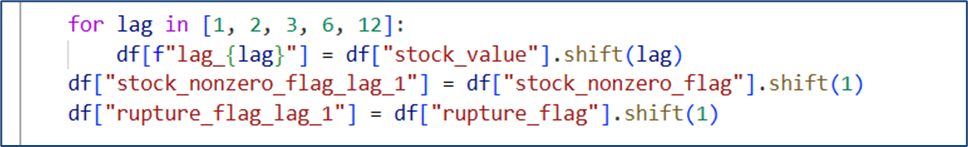
\includegraphics[width=0.9\textwidth]{Figures/Chapitre4/image4.png}
\caption{Extrait du script build_stock_features.py : variables de retard}
\label{fig:ch4: variables de retard}
\end{figure}

L'analyse exploratoire réalisée lors de la phase de compréhension des données a mis en évidence une forte autocorrélation des séries de stock. Cette observation suggère que les valeurs passées contiennent une information particulièrement utile pour prédire les comportements futurs. Les variables de retard constituent donc un élément central du jeu de données utilisé pour l'entraînement des modèles de classification et de régression.
 
Par ailleurs, ces variables jouent un rôle déterminant dans les performances obtenues par les modèles développés dans le cadre de ce projet. Les résultats présentés dans les sections de modélisation montreront que la forte dépendance temporelle observée dans les stocks explique en grande partie la capacité des algorithmes à anticiper les ruptures et à estimer avec précision les niveaux futurs de stock.
 
\paragraph{Les statistiques glissantes (Rolling Features)}\mbox{}\\
 
Les statistiques glissantes consistent à calculer différents indicateurs sur une fenêtre temporelle mobile composée des observations précédentes. Elles permettent de résumer le comportement récent du stock en capturant des notions telles que la tendance, la stabilité, la volatilité ou encore les niveaux extrêmes observés au cours des dernières périodes.
 
Conformément à la stratégie de prévention du Data Leakage adoptée dans ce projet, les statistiques glissantes sont calculées non pas sur la série originale, mais sur la série préalablement décalée à l'aide de la fonction shift(1).
 
\begin{table}[H]
\centering
\caption{Les variables construites : statistiques glissantes}
\label{tab:ch4:rolling_features}
\small
\begin{tabular}{|p{4cm}|p{10cm}|}
\hline
\multicolumn{1}{|c|}{\textbf{Variable}} & \multicolumn{1}{c|}{\textbf{Description}} \\
\hline
Rolling\_Mean\_3 & Moyenne des 3 périodes précédentes \\
\hline
Rolling\_Mean\_6 & Moyenne des 6 périodes précédentes \\
\hline
Rolling\_Mean\_12 & Moyenne des 12 périodes précédentes \\
\hline
Rolling\_Std\_3 & Écart-type des 3 périodes précédentes \\
\hline
Rolling\_Std\_6 & Écart-type des 6 périodes précédentes \\
\hline
Rolling\_Min\_3 & Minimum observé sur les 3 périodes précédentes \\
\hline
Rolling\_Max\_3 & Maximum observé sur les 3 périodes précédentes \\
\hline
\end{tabular}
\end{table}

 \begin{figure}[H]
\centering
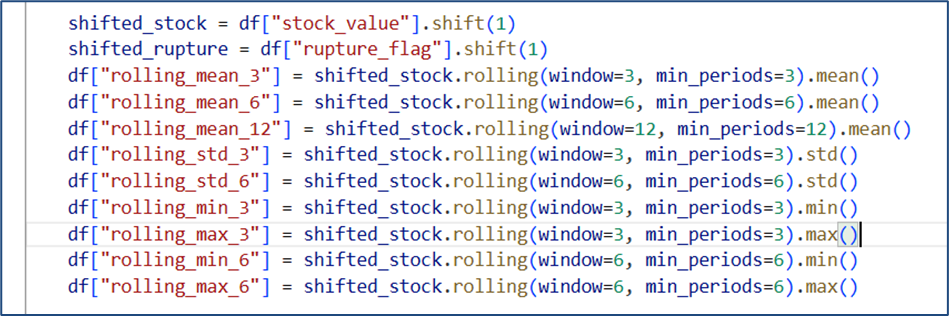
\includegraphics[width=1.1\textwidth]{Figures/Chapitre4/image5.png}
\caption{Extrait du script build_stock_features.py : les statistiques glissantes}
\label{fig:ch4:les statistiques glissantes}
\end{figure}

\textbf{Moyennes glissantes (Rolling Mean)} 
 
Les moyennes glissantes permettent de mesurer la tendance récente du stock en lissant les fluctuations ponctuelles. Trois horizons ont été retenus :
 
\begin{itemize}
    \item Rolling\_Mean\_3 : tendance de court terme 
    \item Rolling\_Mean\_6 : tendance de moyen terme 
    \item Rolling\_Mean\_12 : tendance de long terme
\end{itemize}
 
Par exemple, une valeur faible de Rolling\_Mean\_3 peut signaler une diminution progressive du stock susceptible d'annoncer une future rupture.
 
\textbf{Écart-types glissants (Rolling Standard Deviation)} 
 
Les écarts-types glissants permettent de mesurer la volatilité du stock. Deux horizons ont été retenus :
 
\begin{itemize}
    \item Rolling\_Std\_3
    \item Rolling\_Std\_6
\end{itemize}
 
Une valeur élevée indique que le stock connaît de fortes variations d'une période à l'autre, ce qui peut rendre les prévisions plus complexes et augmenter le risque de rupture. À l'inverse, une faible volatilité traduit généralement un comportement plus stable et plus prévisible.
 
\textbf{Minimums et maximums glissants} 
 
Les indicateurs Rolling\_Min et Rolling\_Max permettent d'identifier les niveaux extrêmes observés récemment. Ces variables apportent une information différente de la moyenne.
 
Par exemple :
 
\begin{itemize}
    \item Un minimum glissant proche de zéro peut indiquer qu'une rupture récente s'est déjà produite ;
    \item Un maximum glissant élevé peut révéler une période de surstockage ou une variation exceptionnelle.
\end{itemize}
 
Ces indicateurs permettent ainsi aux modèles d'identifier les zones de tension ou de stabilité dans l'historique du produit.
 
\paragraph{Les Variables métier}\mbox{}\\
 
Deux produits présentant un niveau de stock similaire peuvent avoir des profils de risque très différents. Un produit ayant connu plusieurs ruptures dans le passé présente généralement une probabilité plus élevée de retomber en rupture qu'un produit historiquement stable. L'intégration de variables métier permet ainsi aux modèles de prendre en compte cette dimension comportementale qui ne peut être capturée uniquement par les variables calendaires ou les statistiques temporelles.
 
Dans ce cadre, quatre variables métier ont été construites :
 
\begin{table}[H]
\centering
\caption{Les variables métier}
\label{tab:ch4:variables_metier}
\small
\begin{tabular}{|p{4cm}|p{9cm}|}
\hline
\multicolumn{1}{|c|}{\textbf{Variable}} & \multicolumn{1}{c|}{\textbf{Description}} \\
\hline
Rupture\_history\_6 & Nombre de ruptures observées durant les 6 dernières périodes \\
\hline
Rupture\_history\_12 & Nombre de ruptures observées durant les 12 dernières périodes \\
\hline
periods\_since\_rupture & Nombre de périodes écoulées depuis la dernière rupture \\
\hline
periods\_since\_nonzero & Nombre de périodes écoulées depuis le dernier stock positif \\
\hline
\end{tabular}
\end{table}

 \begin{figure}[H]
\centering
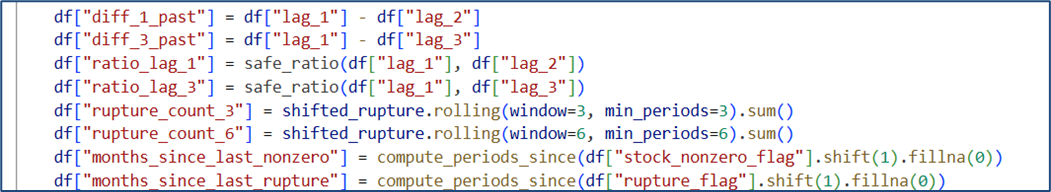
\includegraphics[width=0.9\textwidth]{Figures/Chapitre4/image6.png}
\caption{Extrait du script build_stock_features.py : les variables métier}
\label{fig:ch4:les variables métier}
\end{figure}

\textbf{Historique de rupture} 
 
Les variables rupture\_history\_6 et rupture\_history\_12 mesurent la fréquence des ruptures observées dans le passé récent. Ces variables permettent d'identifier les produits connaissant des ruptures récurrentes. D'un point de vue métier, un produit ayant subi plusieurs ruptures récemment présente généralement un risque plus élevé de connaître de nouvelles tensions d'approvisionnement.
 
\textbf{Nombre de périodes depuis la dernière rupture} 
 
La variable compute\_periods\_since mesure le temps écoulé depuis la dernière rupture observée. Elle permet de représenter la mémoire du système. Un produit sorti récemment d'une rupture peut présenter un comportement différent d'un produit stable depuis plusieurs mois.
 
\textbf{Nombre de périodes depuis le dernier stock positif} 
 
La variable periods\_since\_nonzero mesure le nombre de périodes écoulées depuis la dernière observation présentant un stock strictement positif. Elle est particulièrement utile pour identifier les produits restant durablement en situation de rupture ou les références devenues inactives. C'est-à-dire que si un produit dont le stock est nul depuis plusieurs périodes consécutives présente souvent un comportement différent d'un produit venant ponctuellement de passer à zéro.
 
L'intérêt principal de ces variables réside dans leur capacité à intégrer la dimension opérationnelle du stock. Alors que les variables de retard et les statistiques glissantes décrivent l'évolution quantitative du stock, les variables métier apportent une information qualitative sur la fréquence des ruptures et la stabilité historique des produits.
 
Elles permettent ainsi aux modèles de classification de mieux distinguer les produits présentant un risque élevé de rupture et contribuent à renforcer la pertinence métier des prédictions produites.
 
\subsubsection{Prévention du Data Leakage et validation du Feature Engineering}
 
La qualité d'un modèle prédictif ne dépend pas uniquement des algorithmes utilisés, mais également de la manière dont les données sont préparées. Dans les projets de Machine Learning appliqués aux séries temporelles, l'un des risques méthodologiques les plus importants est le phénomène de Data Leakage (fuite d'information).
 
Le Data Leakage se produit lorsqu'une information issue du futur est involontairement utilisée lors de l'entraînement du modèle. Dans ce cas, les performances obtenues lors de l'évaluation deviennent artificiellement élevées, car le modèle bénéficie d'informations qui ne seraient pas disponibles dans une situation réelle de prédiction.
 
\textbf{Risque de fuite d'information dans les séries temporelles:}
 
Les séries temporelles présentent une particularité importante : les observations sont naturellement ordonnées dans le temps. Contrairement aux problèmes classiques de classification ou de régression, il est impossible d'utiliser des informations provenant de périodes futures pour prédire une période passée.
 
Par exemple, si l'on souhaite prédire le stock d'un produit à la date t, seules les données observées jusqu'à la date t-1 doivent être accessibles au modèle.
 
\textbf{Stratégie de prévention adoptée}
 
Afin d'éviter toute fuite d'information, une règle stricte a été appliquée lors de la construction des variables temporelles : toutes les variables dérivées ont été calculées à partir d'une série préalablement décalée d'une période.
 
Cette approche garantit que les calculs utilisent uniquement les observations disponibles avant la période à prédire.
 
\textbf{Validation de la cohérence des variables construites}
 
Une fois les variables générées, plusieurs contrôles ont été réalisés afin de vérifier leur cohérence et leur compatibilité avec les objectifs du projet.
 
Les vérifications ont notamment porté sur :
 
\begin{itemize}
    \item La présence des variables calculées pour chaque produit.
    \item L'absence d'utilisation d'informations futures.
    \item La cohérence chronologique des observations.
    \item La présence éventuelle de valeurs manquantes générées par les opérations de décalage.
    \item La compatibilité des variables avec les modèles de classification et de régression.
\end{itemize}
 
Les premières observations d'une série temporelle ne disposent pas d'un historique suffisant pour calculer certains indicateurs tels que Lag\_12 ou Rolling\_Mean\_12. Ces observations génèrent naturellement des valeurs manquantes.
 
\subsection{Phase 4 : Modélisation (Modeling)}
 
L'analyse du besoin métier réalisée lors de la phase de Business Understanding a montré que les décideurs doivent répondre à deux questions distinctes mais complémentaires :
 
\begin{itemize}
    \item Un produit risque-t-il de tomber en rupture prochainement ?
    \item Quel sera le niveau de stock futur de ce produit ?
\end{itemize}
 
Ces deux questions correspondent à deux problématiques de Machine Learning différentes. La première consiste à prédire l'apparition d'un événement binaire (rupture ou non-rupture), tandis que la seconde vise à estimer une valeur numérique représentant le niveau futur du stock.
 
Pour répondre à ces besoins, une stratégie de double modélisation a été retenue. Celle-ci repose sur le développement de deux axes analytiques complémentaires :
 
\begin{itemize}
    \item Un axe de classification destiné à prédire le risque de rupture de stock ;
    \item Un axe de régression destiné à estimer les niveaux futurs de stock.
\end{itemize}
 
\subsubsection{Axe 1 : Classification de rupture de stock}
 
La rupture de stock constitue l'un des événements les plus critiques dans la gestion logistique. Elle peut entraîner des retards de livraison, une diminution du niveau de service et une perte de satisfaction des clients. L'identification précoce des produits susceptibles d'entrer en rupture représente donc un enjeu majeur pour l'entreprise.
 
L'objectif de cet axe est de construire un modèle capable de prédire si un produit risque ou non de se retrouver en rupture lors de la période suivante.
 
Le modèle doit produire une sortie binaire permettant d'indiquer si un produit présent ou non un risque de rupture, qui va prendre soit :
 
\begin{itemize}
    \item 0 : absence de risque de rupture ;
    \item 1 : risque de rupture détecté.
\end{itemize}
 
Cette probabilité constitue un élément important pour la priorisation des actions de réapprovisionnement. Un produit présentant une probabilité de rupture de 95\% nécessitera naturellement une attention plus importante qu'un produit dont le risque estimé est de 55\%.
 
Selon James \cite{james2021} : « La classification est une technique d'apprentissage supervisé dont l'objectif consiste à attribuer une observation à une catégorie prédéfinie à partir d'un ensemble de variables explicatives. Dans le cas d'une classification binaire, la variable cible ne peut prendre que deux modalités, représentant généralement la présence ou l'absence d'un événement donné. Cette approche est largement utilisée dans les systèmes d'aide à la décision pour la détection précoce de situations à risque et la prédiction d'événements futurs. » .
 
L'objectif va être de transformer une information historique en un système d'alerte précoce permettant d'anticiper les situations critiques avant leur apparition.
 
\textbf{Sélection et comparaison des modèles de classification}
 
Plusieurs algorithmes de classification ont été évalués afin d'identifier l'approche la plus adaptée aux caractéristiques des données du projet.
 
Le choix d'un modèle ne repose pas uniquement sur ses performances prédictives. Il doit également prendre en compte :
 
\begin{itemize}
    \item La capacité à gérer des relations non linéaires 
    \item La robustesse face au bruit 
    \item La gestion du déséquilibre des classes 
    \item Le temps d'entraînement 
    \item La facilité d'interprétation.
\end{itemize}
 
\begin{table}[H]
\centering
\caption{Les modèles de classification testés}
\label{tab:ch4:modeles_classification}
\small
\begin{tabular}{|p{4cm}|p{10cm}|}
\hline
\multicolumn{1}{|c|}{\textbf{Modèle}} & \multicolumn{1}{c|}{\textbf{Principe}} \\
\hline
Dummy Classifier & Référence aléatoire \\
\hline
Régression Logistique & Modèle linéaire probabiliste \\
\hline
Ridge Classifier & Variante régularisée \\
\hline
Random Forest & Ensemble d'arbres de décision \\
\hline
XGBoost & Gradient Boosting \\
\hline
LightGBM & Gradient Boosting optimisé \\
\hline
\end{tabular}
\end{table}
 
\begin{table}[H]
\centering
\caption{Les résultats obtenus des modèles de classification}
\label{tab:ch4:resultats_classification}
\small
\begin{tabular}{|p{3.5cm}|p{3cm}|p{3cm}|p{3cm}|}
\hline
\multicolumn{1}{|c|}{\textbf{Modèle}} & 
\multicolumn{1}{c|}{\textbf{Accuracy}} & 
\multicolumn{1}{c|}{\textbf{F1-score}} & 
\multicolumn{1}{c|}{\textbf{AUC}} \\
\hline
Dummy & 0,57 & 0,50 & 0,50 \\
\hline
Logistic Regression & 0,80 & 0,70 & 0,75 \\
\hline
Ridge & 0,81 & 0,72 & 0,77 \\
\hline
Xgboost & 0,986 & 0,984 & 0,990 \\
\hline
LightGBM & 0,987 & 0,985 & 0,991 \\
\hline
Random Forest & 0,988 & 0,986 & 0,992 \\
\hline
\end{tabular}
\end{table}
 
Au regard des résultats obtenus, le modèle Random Forest présente les meilleures performances globales et a donc été retenu pour la suite de l'étude.
 
On remarque que parmi les modèles testés, le Random Forest obtient les meilleures performances globales avec :
 
\begin{itemize}
    \item Accuracy = 0,9882
    \item F1-score = 0,9863
    \item AUC = 0,9925
\end{itemize}
 
En plus de ses excellents résultats, ce modèle présente une grande robustesse face aux variables fortement corrélées et aux relations non linéaires observées dans les séries temporelles de stock.
 
Pour ces raisons, le Random Forest a été retenu comme modèle principal de classification.
 
\textbf{Validation temporelle par Expanding Window}
 
Dans un contexte de séries temporelles, l’évaluation des modèles prédictifs doit impérativement respecter la dimension chronologique des données. Contrairement aux méthodes classiques de validation croisée basées sur un découpage aléatoire, ce type de problématique nécessite une approche spécifique afin d’éviter toute fuite d’information (data leakage) entre les ensembles d’entraînement et de test. En effet, l’utilisation de données futures durant la phase d’apprentissage conduirait à des performances artificiellement élevées et à une mauvaise généralisation du modèle en situation réelle.\\
Afin de garantir l’intégrité temporelle des observations, une stratégie de validation de type Expanding Window a été adoptée. Cette approche consiste à entraîner le modèle sur un historique initial, puis à élargir progressivement la fenêtre d’apprentissage au fil du temps tout en évaluant les performances sur des périodes futures jamais observées auparavan.Et au total, 49 folds temporels ont été générés pour la classification.\\
 Cette approche présente plusieurs avantages :
 
\begin{itemize}
    \item Respect de la chronologie réelle 
    \item Simulation fidèle des conditions de production 
    \item Absence de fuite d'information 
    \item Mesure robuste de la stabilité du modèle dans le temps
\end{itemize}

\begin{figure}[H]
\centering

\includegraphics[width=0.9\textwidth]{fig58_validation_temporelle_class.png}
\caption{Extrait du mécanisme de validation temporelle implémenté}
\label{fig:ch4:validation_class}
\end{figure}
 
\paragraph{Résultats de classification}


 
\textbf{Matrice de confusion} 
 
\begin{table}[H]
\centering
\small
\renewcommand{\arraystretch}{1.2}

\caption{Résultats globaux du modèle Random Forest}
\label{tab:ch4:resultats_rf}

\begin{tabular}{|p{4cm}|p{3cm}|}
\hline
\multicolumn{1}{|c|}{\textbf{Métrique}} & \multicolumn{1}{c|}{\textbf{Valeur}} \\
\hline
Accuracy & 0,9882 \\
\hline
Precision & 0,9824 \\
\hline
Recall & 0,9897 \\
\hline
F1-score & 0,9863 \\
\hline
AUC & 0,9925 \\
\hline
\end{tabular}
\end{table}
La matrice de confusion du modèle Random Forest permet d'évaluer la capacité du modèle à distinguer les situations de rupture et de non-rupture. Sur l'ensemble des 99~891 observations évaluées, le modèle identifie correctement 57~305 situations normales (vrais négatifs) et 41~411 situations de rupture (vrais positifs). Les erreurs de classification restent limitées avec seulement 743 faux positifs et 432 faux négatifs.
 
Ces résultats se traduisent par une précision de 98,36\%, un rappel de 98,96\% et un score F1 de 98,63\%. Le faible nombre de faux négatifs est particulièrement important dans un contexte de gestion des stocks, car il signifie que très peu de ruptures réelles échappent à la détection du modèle. De même, le nombre réduit de faux positifs limite les alertes inutiles susceptibles de conduire à des réapprovisionnements excessifs.

\begin{figure}[H]
\centering

\includegraphics[width=0.7\textwidth]{fig59_matrice_confusion.png}
\caption{Matrice de confusion du modèle Random Forest}
\label{fig:ch4:matrice_confusion}
\end{figure}
 
\textbf{Courbe ROC} 
 
L'analyse des prédictions brutes permet de calculer les métriques de performance agrégées sur l'ensemble des folds. Pour évaluer la capacité discriminante du modèle Random Forest retenu, la courbe ROC (Receiver Operating Characteristic) a été tracée en comparant les scores de risque aux labels réels.

\begin{figure}[H]
\centering

\includegraphics[width=0.9\textwidth]{fig60_courbe_roc.png}
\caption{Courbe ROC du modèle Retenu}
\label{fig:ch4:courbe_roc}
\end{figure}

La courbe ROC montre une excellente capacité de discrimination avec une aire sous la courbe (AUC) de 0,9908. Cela est très proche de la valeur optimale, qui est 1. Cela signifie que le modèle Random Forest est très performant pour classer les produits. Il parvient à distinguer avec une grande précision les produits en rupture de stock de ceux qui ne le sont pas. De plus, il minimise les fausses alertes.
 
Pour bien comprendre cela, il faut comparer cette performance à une classification aléatoire. La diagonale grise sur la courbe ROC représente une telle classification. Dans ce cas, l'AUC serait de 0,5. La différence entre les deux valeurs est donc très significative. Cela met en évidence l'importance des variables temporelles et logistiques utilisées par le modèle Random Forest. Ces variables sont donc très pertinentes pour prédire les ruptures de stock.
 
En complément de la courbe ROC, les métriques de performance consolidées du modèle Random Forest confirment son excellente capacité prédictive. Sur l'ensemble des 49 folds de validation temporelle, le modèle atteint un F1-score de 0,986, une précision de 0,983 et un rappel de 0,989. Ces résultats témoignent d'un équilibre remarquable entre la détection des ruptures réelles et la limitation des fausses alertes, validant ainsi le choix du Random Forest comme modèle de référence pour la classification de rupture.
 
Sur le plan opérationnel, ces performances signifient que le modèle est capable d'identifier plus de 98\% des produits à risque de rupture tout en maintenant un taux de fausses alertes inférieur à 2\%. Cette fiabilité permet aux responsables logistiques de prioriser leurs actions de réapprovisionnement avec un niveau de confiance élevé.
 
\textbf{Analyse des performances} 
 
Les résultats obtenus montrent que le modèle Random Forest est particulièrement performant pour la prédiction des ruptures de stock. Avec une accuracy de 98,82\%, un score F1 de 98,63\% et une AUC de 0,9925, le modèle parvient à distinguer efficacement les situations de rupture des situations normales.
 
L'analyse de la matrice de confusion révèle un nombre très élevé de prédictions correctes, avec 57~305 vrais négatifs et 41~411 vrais positifs, contre seulement 743 faux positifs et 432 faux négatifs. Ces résultats traduisent une excellente capacité de détection des ruptures tout en limitant les fausses alertes.
 
Les performances observées peuvent s'expliquer par la forte dépendance temporelle des niveaux de stock. Les variables construites à partir de l'historique (lags, statistiques glissantes et indicateurs métier) capturent efficacement les comportements récurrents présents dans les données.
 
\subsubsection{Axe 2 : Régression du stock}
 
Si la classification permet d'identifier l'existence d'un risque de rupture, elle ne quantifie pas l'ampleur de ce risque. C'est pourquoi ce deuxième axe analytique complémentaire a été développé : la régression du stock, qui vise à estimer la valeur future du niveau de stock pour chaque produit.
 
C'est-à-dire que si la classification répond à la question « Ce produit va-t-il tomber en rupture ? », la régression vise à quantifier « Quel sera le niveau de stock de ce produit sur un horizon donné ? »
 
L'objectif du modèle est de produire une sortie continue représentant la valeur prédite du stock (stock\_value) sur un horizon de 1 à 3 mois :
 
\begin{itemize}
    \item Sortie : valeur numérique continue (quantité de stock prévue) ;
    \item Unité : nombre d'unités de produit.
\end{itemize}
 
Selon Montgomery Peck et Vining \cite{montgomery2021}: « la régression constitue une méthode statistique et d’apprentissage supervisé permettant de modéliser la relation entre une variable quantitative à prédire et un ensemble de variables explicatives. Son objectif est d'estimer la valeur future d'une variable continue en exploitant les relations observées dans les données historiques. Cette approche est largement utilisée dans les domaines de la prévision et de l'aide à la décision en raison de sa capacité à fournir des estimations quantitatives directement exploitables par les gestionnaires » 
 
Cette logique de régression constitue le second composant analytique du futur système décisionnel intelligent et sera intégrée dans l'application finale aux côtés de la classification.
 
\textbf{Sélection et comparaison des modèles de régression}
 
Plusieurs modèles de régression ont été évalués afin d'identifier l'approche la plus adaptée aux caractéristiques des données de stock. Les expérimentations ont notamment porté sur un modèle naïf (Naive Baseline), une régression Ridge ainsi qu'un modèle Random Forest Regressor.
 
L'évaluation des performances a été réalisée à l'aide des métriques classiques de régression, notamment le coefficient de détermination (R²), l'erreur absolue moyenne (MAE) et la racine de l'erreur quadratique moyenne (RMSE).
 
\textbf{Comparaison des modèles de régression}
 \renewcommand{\arraystretch}{1.2}
\begin{table}[H]

\centering
\caption{Comparaison des modèles de régression}
\label{tab:ch4:comparaison_regression}
\small
\begin{tabular}{|p{4.5cm}|p{12cm}|}
\hline
\multicolumn{1}{|c|}{\textbf{Modèle}} & \multicolumn{1}{c|}{\textbf{Principe}} \\
\hline
Naive Baseline & La prédiction correspond à la dernière valeur de stock observée. Autrement dit, le stock futur est supposé identique au stock actuel. \\
\hline
Ridge Regression & Modèle linéaire qui estime le stock futur à partir d'une combinaison pondérée des variables explicatives tout en appliquant une régularisation pour limiter le surapprentissage. \\
\hline
Random Forest Regressor & Ensemble d'arbres de décision construits sur différents échantillons des données. La prédiction finale correspond à la moyenne des prédictions produites par les arbres. \\
\hline
\end{tabular}
\end{table}
 \renewcommand{\arraystretch}{1.2}
\begin{table}[H]
\centering
\caption{Les résultats obtenus des modèles de régression}
\label{tab:ch4:resultats_regression}
\small
\begin{tabular}{|p{4cm}|p{3cm}|p{3cm}|}
\hline
\multicolumn{1}{|c|}{\textbf{Modèle}} & 
\multicolumn{1}{c|}{\textbf{R²}} & 
\multicolumn{1}{c|}{\textbf{MAE}} \\
\hline
Naive Baseline & 0,9759 & 533,8 \\
\hline
Random Forest & 0,9398 & 1467,4 \\
\hline
Ridge Regression & 0,9121 & 1823,7 \\
\hline
\end{tabular}
\end{table}
 
Les résultats obtenus montrent que le modèle Naïve Baseline présente les meilleures performances parmi les approches évaluées, avec un coefficient de détermination (R²) de 97,59\% et une erreur absolue moyenne (MAE) de 533,8 unités. Les modèles Random Forest et Ridge Regression obtiennent également des performances satisfaisantes, mais restent inférieurs à cette approche de référence.
 
Cette observation s'explique par la forte dépendance temporelle des niveaux de stock. En effet, dans de nombreux cas, le stock observé à une période donnée demeure proche de celui de la période précédente. Dans ce contexte, l'hypothèse du modèle Naïve, qui consiste à considérer que la prochaine valeur sera identique à la dernière valeur observée, constitue déjà une approximation très efficace.
 
Ces résultats mettent en évidence l'importance de l'autocorrélation dans les séries de stock étudiées et montrent que la complexité d'un modèle n'entraîne pas systématiquement une amélioration des performances prédictives.
 
\textbf{Validation temporelle par Expanding Windows}
 
Afin de garantir la cohérence méthodologique avec l'axe de classification, la validation du modèle de régression a également été réalisée selon une stratégie d'Expanding Window.
 
À chaque itération, le modèle est entraîné sur l'ensemble des observations disponibles jusqu'à une date donnée puis évalué sur la période immédiatement suivante. Cette approche respecte la chronologie des données et reproduit fidèlement les conditions réelles d'utilisation du modèle.
 
Dans le cadre de ce projet, la procédure de validation a généré 61 folds temporels, permettant d'évaluer la robustesse du modèle sur différentes périodes de l'historique disponible.

\begin{figure}[H]
\centering

\includegraphics[width=0.9\textwidth]{fig61_validation_temporelle_reg.png}
\caption{Extrait du mécanisme de validation temporelle implémenté dans le modèle de régression}
\label{fig:ch4:validation_reg}
\end{figure}
 
\textbf{Résultats de régression}
 
L'évaluation du modèle retenu montre des performances particulièrement satisfaisantes pour l'estimation des niveaux futurs de stock.
 
Les principaux résultats obtenus sont les suivants :
 
\begin{table}[H]
\centering
\caption{Les résultats obtenus du modèle Naive Baseline}
\label{tab:ch4:resultats_naive}
\small
\begin{tabular}{|p{4cm}|p{3cm}|}
\hline
\multicolumn{1}{|c|}{\textbf{Métrique}} & \multicolumn{1}{c|}{\textbf{Valeur}} \\
\hline
R² & 0,9759 \\
\hline
MAE & 533,8 \\
\hline
RMSE & 11~623,9 \\
\hline
\end{tabular}
\end{table}
 
L'analyse des résultats confirme que les niveaux de stock présentent une forte stabilité temporelle. Le modèle Naïve Baseline parvient ainsi à expliquer près de 98\% de la variance observée, ce qui traduit une forte persistance des valeurs de stock d'une période à l'autre.
 
Malgré des performances légèrement inférieures, les modèles Random Forest et Ridge Regression demeurent capables de capturer une grande partie de la dynamique du stock. Toutefois, le gain apporté par ces approches plus sophistiquées reste limité face à la simplicité et à l'efficacité du modèle de référence.
 
D'un point de vue opérationnel, ces résultats montrent que l'évolution du stock est largement déterminée par son historique récent. Ils confirment également la pertinence des variables temporelles construites lors de la phase de préparation des données et valident la faisabilité d'une approche prédictive appliquée à la gestion des stocks.
 
\subsection{Phase 5 : Évaluation}
 
Les deux axes Data Science développés dans ce projet constituent des approches complémentaires pour anticiper et gérer les risques logistiques. Bien qu'ils reposent sur les mêmes données historiques issues de Fact\_Stock et suivent un protocole de validation temporelle identique (expanding window), ils répondent à des questions métier distinctes et mobilisent des méthodologies différentes.
 
Cette phase vise non seulement à analyser les performances techniques des modèles, mais également à examiner leur pertinence opérationnelle dans le contexte de la gestion des stocks de BIOSPHERE, mais aussi de déterminer dans quelle mesure les résultats obtenus peuvent contribuer à l'amélioration du processus de réapprovisionnement et à la réduction des risques de rupture.
 
\subsubsection{Évaluation de l'axe Classification}
 
Le premier axe du projet avait pour objectif d'anticiper les situations de rupture de stock à travers un problème de classification binaire. Les résultats obtenus montrent que les modèles développés atteignent des performances élevées en termes d'Accuracy, Precision, Recall et ROC-AUC.
 
Le modèle retenu est capable d'identifier efficacement les situations à risque tout en limitant les faux positifs. Cette capacité de détection précoce constitue un apport significatif pour les responsables du stock, qui peuvent ainsi anticiper les besoins de réapprovisionnement avant l'apparition effective des ruptures.
 
\subsubsection{Évaluation de l'axe Régression}
 
Le second axe du projet visait à estimer les niveaux futurs de stock à travers un problème de régression. Les résultats montrent que les différents modèles testés sont capables de reproduire correctement l'évolution des niveaux de stock.
 
L'évaluation a mis en évidence la forte autocorrélation des séries temporelles étudiées, ce qui explique les excellentes performances du modèle Naïve Baseline utilisé comme référence. Malgré cela, les modèles de Machine Learning ont également démontré leur capacité à capturer les tendances générales des stocks et à fournir des estimations fiables.
 
\subsubsection{Comparaison méthodologique et performances des deux axes}
 
\begin{table}[H]
\centering
\caption{Comparaison méthodologique et performances}
\label{tab:ch4:comparaison_axes}
\small
\begin{tabular}{|p{3.5cm}|p{5.5cm}|p{5.5cm}|}
\hline
\multicolumn{1}{|c|}{\textbf{Critère}} & \multicolumn{1}{c|}{\textbf{Classification de rupture}} & \multicolumn{1}{c|}{\textbf{Régression du stock}} \\
\hline
Nature du problème & Classification binaire supervisée & Régression supervisée \\
\hline
Meilleur modèle & Random Forest & Naive Baseline \\
\hline
Configuration optimale & feature\_set=reduced, horizon=1, scope=all\_products & feature\_set=baseline, horizon=1, scope=all\_products, target\_transform=raw \\
\hline
Hyperparamètres clés & n\_estimators=140, max\_depth=8, class\_weight=balanced\_subsample & Report de la dernière observation (y\_pred = y\_{t-1}) \\
\hline
Métrique principale & F1-score = 0,986294 & R² = 0,975963 \\
\hline
Métriques secondaires & Accuracy = 0,988230, Precision = 0,983575, Recall = 0,989644, ROC-AUC = 0,992451 & MAE = 533,79, RMSE = 11~623,95 \\
\hline
\end{tabular}
\end{table}
 
\subsubsection{Limites du projet et perspectives d'amélioration}
 
Les résultats obtenus dans les deux axes de ce projet démontrent la pertinence d'une approche Data Science appliquée à la gestion prévisionnelle des stocks. Les modèles développés ont permis, d'une part, d'anticiper les risques de rupture de stock grâce à une approche de classification performante et, d'autre part, d'estimer l'évolution future des niveaux de stock à travers un modèle de régression adapté aux caractéristiques des données étudiées. Les performances observées confirment ainsi la faisabilité technique et opérationnelle d'un système prédictif capable d'apporter une aide à la décision dans le domaine de la gestion logistique.
 
Les résultats particulièrement élevés obtenus lors de la phase de modélisation, notamment pour la classification des ruptures de stock, peuvent s'expliquer par la forte dépendance temporelle observée dans les séries de stock. Les variables construites à partir de l'historique des mouvements, telles que les retards temporels (lags), les statistiques glissantes et les indicateurs métier, permettent de capturer efficacement les comportements récurrents des produits. Cette richesse informationnelle contribue directement aux excellentes performances obtenues par les algorithmes de Machine Learning. Toutefois, ces résultats doivent être interprétés dans le contexte spécifique de l'entreprise BIOSPHERE et mériteraient d'être validés sur des périodes supplémentaires ainsi que sur d'autres environnements logistiques afin de confirmer leur capacité de généralisation.
 
Par ailleurs, les modèles développés reposent essentiellement sur l'exploitation de données internes liées aux mouvements de stock. Bien que ces informations se soient révélées particulièrement pertinentes, l'intégration future de variables externes pourrait permettre d'améliorer davantage la précision des prédictions. Parmi les pistes envisageables figurent notamment l'intégration des prévisions de ventes, des délais fournisseurs, des campagnes promotionnelles, des événements saisonniers ou encore de certains indicateurs économiques susceptibles d'influencer la demande et les besoins d'approvisionnement.
 
Une autre limite du projet concerne la valorisation opérationnelle des résultats produits. À ce stade, les prédictions générées par les modèles demeurent sous forme de sorties analytiques produites dans l'environnement de développement Data Science. Les indicateurs prédictifs obtenus ne sont pas encore directement accessibles aux utilisateurs métiers à travers une interface dédiée leur permettant d'exploiter facilement les informations générées.
 
Dans une perspective d'amélioration, il serait particulièrement pertinent de mettre en place une plateforme décisionnelle intégrée permettant de centraliser les résultats des analyses descriptives issues de la Business Intelligence et les prédictions produites par les modèles de Machine Learning. Une telle solution offrirait aux responsables logistiques une vision globale de la situation actuelle des stocks ainsi qu'une capacité d'anticipation des risques futurs. L'intégration de tableaux de bord interactifs, d'indicateurs de risque de rupture, de mécanismes d'alerte automatique et de scénarios de réapprovisionnement constituerait une évolution naturelle du système développé.
 
Enfin, une étape supplémentaire pourrait consister à industrialiser le cycle complet de prédiction à travers la mise en place d'un processus automatisé de mise à jour des données, de réentraînement périodique des modèles et de génération continue des prévisions. Cette approche permettrait de garantir la pérennité des performances obtenues tout en assurant une adaptation permanente du système aux évolutions de l'activité de l'entreprise.
 
Ces différentes perspectives s'inscrivent pleinement dans la phase de déploiement de la méthodologie CRISP-DM, dont l'objectif final est de transformer les résultats analytiques et prédictifs obtenus en un véritable outil décisionnel intelligent capable de soutenir durablement les processus de gestion, de planification et de réapprovisionnement de l'entreprise.
 
\section{Conclusion}
 
Dans ce chapitre, nous avons appliqué la méthodologie CRISP-DM afin de développer une solution prédictive dédiée à la gestion des stocks de BIOSPHERE. Après les phases de compréhension métier, d'analyse et de préparation des données, deux axes de modélisation ont été mis en œuvre : la prédiction du risque de rupture de stock par classification et l'estimation des niveaux futurs de stock par régression.
 
Les résultats obtenus confirment la pertinence des approches retenues et démontrent la possibilité de passer d'une analyse descriptive à une démarche prédictive permettant d'anticiper les situations critiques. Toutefois, les prédictions générées restent à ce stade sous forme de résultats analytiques. Leur valorisation opérationnelle nécessite désormais une phase de déploiement et d'intégration dans un environnement décisionnel adapté, qui fera l'objet du chapitre suivant.